\documentclass[a4paper,onecolumn,11pt]{article}
%%%%
\renewcommand{\familydefault}{\sfdefault}%
%%%

%Packages%%%%%%%%%%%%%%%%%%%%
\usepackage[margin=2cm]{geometry} %this aasures 2cm margin on all sides
\usepackage{graphicx}% to include figures
\usepackage{array}%
\usepackage{url}%
\usepackage{hyperref}

\usepackage{graphicx}  % For including images
\usepackage{float}     % For the [H] placement option

\hypersetup{linkcolor=blue, pdftitle={title for PhD Research Proposal}, pdfauthor={Babu Pallam}, pdfsubject={Research Proposal Condensed -- May 2024}, pdfkeywords={keyword1, keyword2, keyword3} }
%%%%%%%%%%%%%%%%%%%%%%%%%%%%%%%%%%%%%%%%%%%%%%%%%%%%%%%%%%%%%%%%%%%%%%%%%%%%%%%%%%%%%%%%%%%%%%%%%%%%%%%%%%%%%%%%%%%%%%%%%%%%%%%%%%%%%%%%%%%%%%%%%%%%%%%%%%%%%%%%%%%%%%%%%%
%%DOUBLE QUOTE and SINGLE QUOTE Commands%
\newcommand{\qq}[1]{\textquotedblleft#1\textquotedblright}%
\newcommand{\q}[1]{\textquoteleft#1\textquoteright}%
%%%%%%%%%%%%%%%%%%%%%%%%%%%%%%%%%%%%%%%%%%%%%%%%%%%%%%%%%%%%%%%%%%%%%%%%%%%%%%%%%%%%%%%%%%%%%%%%%%%%%%%%%%%%%%%%%%%%%%%%%%%%%%%%%%%%%%%%%%%%%%%%%%%%%%%%%%%%%%%%%%%%%%%%%%
\pagenumbering{arabic}%
%\setcounter{page}{-1}%
%%%%%%%%%%%%%%%%%%%%%%%%%%%%%%%%%%%%%%%%%%%%%%%%%%%%%%%%%%%%%%%%%%%%%%%%%%%%%%%%%%%%%%%%%%%%%%%%%%%%%%%%%%%%%%%%%%%%%%%%%%%%%%%%%%%%%%%%%%%%%%%%%%%%%%%%%%%%%%%%%%%%%%%%%
\begin{document}
%%%%%%%%%%%%%%%%%%%%%%%%%%%%%%%%%%%%%%%%%%%%%%%%%%%%%%%%%%%%%%%%%%%%%%%%%%%%%%%%%%%%%%%%%%%%%%%%%%%%%%%%%%%%%%%%%%%%%%%%%%%%%%%%%%%%%%%%%%%%%%%%%%%%%%%%%%%%%%%%%%%%%%%%%%
\title{Enhancing Sentiment Analysis Accuracy through Contextual Understanding in Social Media Texts}
\author{\textbf{Babu Pallam}\\
MSc Artificial Intelligence,\\ De Montfort University, Leicester
}%
%%%%%%%%%%%%%%%%%%%%%%%%%%%%%%%%%%%%%%%%%%%%%%%%%%%%%%%%%%%%%%%%%%%%%%%%%%%%%%%%%%%%%%%%%%%%%%%%%%%%%%%%%%%%%%%%%%%%%%%%%%%%%%%%%%%%%%%%%%%%%%%%%%%%%%%%%%%%%%%%%%%%%%%%%%
% make the title area
\maketitle
\thispagestyle{empty}
%%%%%%%%%%%%%%%%%%%%%%%%%%%%%%%%%%%%%%%%%%%%%%%%%%%%%%%%%%%%%%%%%%%%%%%%%%%%%%%%%%%%%%%%%%%%%%%%%%%%%%%%%%%%%%%%%%%%%%%%%%%%%%%%%%%%%%%%%%%%%%%%%%%%%%%%%%%%%%%%%%%%%%%%%%
%%%%%%%%%%%%%%%%%%%%%%%%%%%%%%%%%%%%%%%%%%%%%%%%%%%%%%%%%%%%%%%%%%%%%%%%%%%%%%%%%%%%%%%%%%%%%%%%%%%%%%%%%%%%%%%%%%%%%%%%%%%%%%%%%%%%%%%%%%%%%%%%%%%%%%%%%%%%%%%%%%%%%%%%%%
\section{Summary}
Sentimental analysis has become one of the most important subject areas in Artificial Intelligence(AI) which has been widely popular in the research community. Sentiment analysis enables us to decode human emotions and opinions from the data, which is produced as a result of user interactions on social media platforms, and draws inferences that is useful in various domains. Machine learning and Natural Language Processing(NLP) techniques has enabled us to do extensive research and thoughts into this area which does automate the Sentiment Analysis for leveraging the present challenges exist in the respected domains. Sentiment analysis has been narrowed down in this report as a component of NLP. With the help of algorithms, it does automatically analyse and extract subjective information from data which can be considered as an output of opinion, review, or emotion of the individuals. 
However, the accuracy of the implementations of Sentiment Analysis had brought significant concerns and challenges. For instance, handling of slang, emojis according to the trend and mix of culture, mixed language notation, and several others. At present, in the world of Internet, where tons of data is being generated in every moment, on different social and economic web platforms, existing sentiment analysis models often finds it difficult to capture the sentiments expressed by the people, in terms of politics, economic, and social values. Thereby, the importance of doing research is not negligible, and can cause a significant impact in the future.

The succinct outline of the proposed research is as follows. The proposed research aims to address the limitations of existing sentiment analysis models by increasing the accuracy of social media texts. Through the advancement of technology in Artificial Intelligence, such as natural language processing, machine  learning algorithms, and deep learning algorithms, this research focuses on designing  and developing novel methodologies for improving the accuracy of data that is being generated on the Internet. This research begins with exploring the existing methodologies which lies behind the integration available and used on the Internet for capturing sentiments, social network analysis and sentiments expressed in the social media posts. In addition to this, as a second step, the research will investigate the productiveness of transfer learning techniques, which is the most vanilla concept in Deep learning, while using those pre-trained models across different domains.  In addition, this research aims to design a methodology, which would be more towards experimental, that has got more advancements in Sentimental Analysis accuracy. Thereby, this research provides more insights for monitoring strategies for social media, along with the theme of applying these insights into different domains including economic market analysis, e-commerce platforms and others.


%%%%%%%%%%%%%%%%%%%%%%%%%%%%%%%%%%%%%%%%%%%%%%%%%%%%%%%%%%%%%%%%%%%%%%%%%%%%%%%%%%%%%%%%%%%%%%%%%%%%%%%%%%%%%%%%%%%%%%%%%%%%%%%%%%%%%%%%%%%%%%%%%%%%%%%%%%%%%%%%%%%%%%%%%%

%%%%%%%%%%%%%%%%%%%%%%%%%%%%%%%%%%%%%%%%%%%%%%%%%%%%%%%%%%%%%%%%%%%%%%%%%%%%%%%%%%%%%%%%%%%%%%%%%%%%%%%%%%%%%%%%%%%%%%%%%%%%%%%%%%%%%%%%%%%%%%%%%%%%%%%%%%%%%%%%%%%%%%%%%%

\section{Background}

Sentiment analysis, the sub-field of Natural Language Processing (NLP), aims to automate the process of identifying and extracting subjective information from texts. Which includes the opinions, emotions, attitudes, and views. Recent years have brought significant attention for Sentiment analysis because of its application possibility in various domains, including marketing, customer feedback management, political analysis, brand reputation management, site engine optimization, and others. Capturing accurate sentiments from the social media text is quite challenging because of the characteristics of data such as use of informal language, linguistic variations, identifying contextual meaning of the data, and several others.
 Use of traditional machine learning algorithms for sentiment analysis is the beginning of today’s advancement in this area. Which uses annotated datasets does based on the lexical analysis for identifying the sentiments from the data. Bo Pang in 2002 \cite{pang2002thumbs}, provides an insights of how sentiment classification can be done using ML algorithms. This paper discusses about the effectiveness of those algorithms. 

ML approach was promising, but challenges were exist which should be solved, including lack of robustness, and high noise while dealing with dynamic environments of social media. Middleman inter-mediation in analysing the data was crucial in this approach since the accuracy was not enough to go forward with the inferences made by the system. To address these challenges, there are several explorations carried out by researchers over various methodologies in the recent years. Among different areas of texts analysis, contextual understanding of the text is very important. Contextual understanding means the ability of a computational system to automatically comprehend and interpret the information or sentiment behind the text based on the context.  It includes the syntax of the text, user interaction pattern, the general context sentiment, and others. Recent advancements in Deep Learning, especially concepts of Transformers and GPT, has leveraged the performance and potential of sentiment analysis on different domains.  Other models available are such as, ELMo (Embedding from Language Models)\cite{ilic2018deep}, BERT (Bidirectional Encoder Representations from Transformers) \cite{devlin2018bert}, RoBERTa (Robustly Optimized BERT Pretraining Approach)\cite{liu2019roberta}, and XLNet\cite{yang2019xlnet}. Apart from this, several approaches that integrates domain specific models have been proposed and found the implementations in several domains at present.  For instance, Tang et al. proposed a sentiment analysis framework \cite{tang2015effective} that uses user social network information to enhance sentiment prediction accuracy. 


Overall, this literature review highlights the importance of enhancing the accuracy of sentiment analysis through the contextual understanding of social media texts. The recent advancement in this area has shown the promising results of this and the versatility of domains where it can be applied. Based on the limitations exist in this in terms of improving accuracy while handling human sarcasm, irony, and other way of interactions, the topic chosen in this research proposal is worthful for a research and exploration. Thereby, the proposed research aims to contribute an extended boundary or creating a new edge for existing research.


\section{Proposed Work}
\subsection{Aims and Objectives}
Which includes the aim of the research, and the objectives foreseen to be satisfied throughout the research
\subsubsection{AIM: }
	The aim of this research is to improve the effectiveness and accuracy of sentiment analysis in social media texts through contextual understanding, which indirectly strengthen the NLP techniques.
\subsubsection{Objectives: }
\begin{itemize}
  \item{To investigate existing integration of sentiment analysis for contextual understanding in social media texts}
	\begin{enumerate}
	    \item{Investigate existing contextual embedding models (e.g., BERT, ELMo) in capturing contextual information from social media texts.}
	    \item{Compare the accuracy achieved by the models against traditional approaches, such as ML algorithms and rule-based approaches.}
	    \item{Explore and Analyse the impact of different contextual embedding architectures (e.g., bidirectional, transformer-based) on sentiment analysis performance.}
	\end{enumerate}
  \item{To gather transfer learning techniques for domain adaptation in sentiment analysis across different social media platforms.}
	\begin{enumerate}
	    \item{Collect datasets from diverse social media platforms (eg: Twitter, Facebook, and Instagram).}
	    \item{Explore different transfer learning approaches (e.g., fine-tuning, domain adversarial training) for analysis of performance of different platforms.}
	\end{enumerate}
  \item{To design and develop a methodology for enhancing sentiment analysis accuracy in social media texts.}
	\begin{enumerate}
	    \item{Design a sentiment analysis framework combining the concepts of contextual embedding, user context, and transfer learning techniques .}
	    \item{Implement the proposed framework using state of art NLP libraries and frameworks (e.g., TensorFlow, PyTorch).}
	    \item{Evaluate the performance of the framework proposed in terms of accuracy.}
	\end{enumerate}
\end{itemize}
By achieving the objectives, the research put forward a clear understanding of state of art sentiment analysis models, the concepts involved in it, the existing contextual embedded models, different between the models, and development of a new improved sentiment analysis model.

\subsection{Rationale}

The importance of sentiment analysis in social media is worth to be investigated. At present, the social media platforms have become the primary space on the Internet for individuals to express their own opinions and emotions on diverse topics from brand to politics, from personnel to social. 

So, analysing these responses based on the specific domain can provide valuable insights to various domains, for example, businesses, researchers, and government. But the accurate processing of data to understand the exact meaning of what the sentence must be meant in the specific context and the automation of the processing to avoid human error and bias became a challenge which put forward the scope of further research in this area. Recent developments in NLP and Deep learning demonstrated different contextual embedding models which can solve these challenges. Enhancing the performance of those models or extending the existing models with additional functionalities are important where research should be focused on. So, the time this research has been proposed is found to be the perfect time. 

To conclude, enhancing sentiment analysis accuracy by proposing new methodologies through contextual understanding in social media texts is essential to extend the features and unlock the capabilities of sentiment analysis in today’s digital age. By addressing the challenges exist right now, this research can contribute more advancement in the field of NLP. 


\section{Methodology}

The methodology involves 5 steps as given below.
\begin{enumerate}
  \item \textbf{Literature Review:} The methodology prepared to do this research begins by conducting research on the existing contextual embedded models available now and the recent research going in this area. This comes under literature review part. After the qualitative research done in this area the challenges and the possibilities should be formulated. Then based on these formulated points, the next step begins. 
  \item \textbf{Data Collection:} In which collecting diverse dataset of social media texts from different popular platforms Twitter, Facebook, Reddit, and Instagram. These platform associated data, including personnel messages, blogs, discussions and others, must be comprised of various topics, languages, and user profiles, and user interactions.
  \item \textbf{Preprocessing:}  cleaning the data, including removing null characters, tokenization, normalizing texts, and others. 
  \item \textbf{Model Development:} in this step, based on the data processed, develop a sentiment analysis model based on deep learning architecture like Recurrent Neural Networks(RNN) or Convolutional Neural Networks (CNN). Integrate pre-trained models along with this for comparing and optimizing the model.
\item \textbf{Evaluation Metrics:} analyse the performance of this model using  standard evaluation metrics such as accuracy, precision, recall, and F1-score.
\end{enumerate}


\section{Work Packages}

The objective of research has been decomposed into 4 steps.
\begin{enumerate}
  \item \textbf{Work Package 1: Literature Review:} This package’s aim is fulfilling the first objective mentioned in section 3.1.2. The tasks to be performed are as follows: a) review the fundamental concepts of sentimental analysis, b) review the papers that present the traditional approaches that had been used for sentimental analysis, which include, Naïve Bayes, Support Vector Machine, and Decision Trees. c)review the contextual embedded models and d) summarise after the comparison of the models into limitations and challenges of the existing models which would open the space for further research. The estimated time required is approximately 12 months. 

  \item \textbf{Work Package 2:  Data Collection and Preprocessing: }  This includes collection of data from different social media platforms and process those data according to the input pattern required for our proposed model, which is specified as objective 2 in section 3.1.2. The tasks involved are as follows: a) Identify relevant social media platforms (e.g., Twitter, Facebook, Reddit), b) use web scrapers or on request with platform providers to collect the large dataset required from different social platforms, c) process the data by tokenizing texts, removing noise, and normalization. The estimated time required is approximately 6 months.
  \item \textbf{Work Package 3: Model Development and Training:}  Design and implement sentiment analysis models based on deep learning architecture, specified as third objective in section 3.1.2. The tasks involved are as follows: a) implement model using RNN or CNN, b) experiment with different variations and parameter values, c) find specific combinations of values that can improve results, and d) train the model using pre-processed data specified in package 2. The estimated time required is approximately 6 months.

  \item \textbf{Work Package 4: Model Development:} This relates to the objective 3 specified in section 3.1.2.  The main aim of this package is the evaluation of the performance of model designed in order to optimize accuracy. Tasks involves are as follows: a) evaluate using evaluation metrics such as accuracy, precision, and F1-score, 2) optimize model hyper-parameters to improve accuracy of the model implemented. The estimated time required is approximately 12 months.
\end{enumerate}

By breaking down the project into four packages, which are directly associated with the objective specified in section 3.2, the research can be done smoothly, ensuring that each objective is fulfilled at the end.

%%%%%%%%%%%%%%%%%%%%%%%%%%%%%%%%%%%%%%%%%%%%%%%%%%%%%%%%%%%%%%%%%%%%%%%%%%%%%%%%%%%%%%%%%%%%%%%%%%%%%%%%%%%%%%%%%%%%%%%%%%%%%%%%%%%%%%%%%%%%%%%%%%%%%%%%%%%%%%%%%%%%%%%%%%
\vspace{15pt}
%%%%%%%%%%%%%%%%%%%%%%%%%%%%%%%%%%%%%%%%%%%%%%%%%%%%%%%%%%%%%%%%%%%%%%%%%%%%%%%%%%%%%%%%%%%%%%%%%%%%%%%%%%%%%%%%%%%%%%%%%%%%%%%%%%%%%%%%%%%%%%%%%%%%%%%%%%%%%%%%%%%%%%%%%%


\section{Professional, Legal, and Ethical Issues}

	Since this research discuss about the accuracy of sentiment analysis of existing models and proposing a new model to enhance the accuracy of sentiment analysis, the professional, legal and ethical issues should be taken into account.

\textbf{Professional Considerations:}
	During the research, it is important to keep professional values, in each stage of the research. The literature review involve the protocol of keeping appreciation and value of other peoples’ work. The research methodology involves certain criteria which is considered as best practice to improve the efficiency of the model. While developing and implementing the model, the collaborations with peers, mentors, and experts from the external fields is significant to improve the research process. In addition, publishing papers contribute to the community of research about the state of art knowledge is part of being professional. 

\textbf{Legal Considerations:}
	This include the privacy and authenticity of work. During the literature review phase, the unauthorized use of papers, and stating unrecognized data as truth according to the convenience of the research proposed should not be performed. Research should be based on legal documents and legal data, which involved in data collection process too. The data should be collected from authentic resources, which should be based on relevant data protection laws under government rules. Giving appreciation to use of other persons resources should be always taken into consideration.

\textbf{Ethical Considerations:}
	The research involved data collection. The researcher must honour the users privacy and consent prior to data collection. This involves clear communication with the social-media platform providers how the data is being used and how their data will be protected. Another important aspect should be considered is the bias and fairness of data. The researcher should be modelling the problem enduring the fair treatment to every individual’s data.


\section{Relevance to Beneficiaries}

The research to be carried out will benefit two domains, such as economic and social domains. These two are discussed below.

\textbf{Economic Impact:}
	A small improvement in the accuracy could result into a significant change in the insight that a sentimental analysis model can provide into the problem or response irrespective of the domain specification. Hence, the beneficiaries of this research are several. Some of them are mentioned in this section. A major impact can be made in the case of business and marketing professionals. The improved sentiment analysis accuracy enables the individuals in this field to gain more comprehensive insights into customer responses. The businesses can identify the trends, the perception of brands and taste of customers, which enables then to understand and optimize the marketing strategies for better growth. This will help them to maintain the reputation of the business too. In the field of marketing, the enhanced model can make same effect. The insights about the consumer sentiments, competitions exist, and others would help them to take actions for better decision making and strategic planning. 

\textbf{Social Impact:}

	The social impact of this research has been seen over several domains. Some of them are as follows. First, the public opinion monitoring for administrative systems. The enhance accuracy of model contributes a better understanding of public opinion over social issues or social impacts, including cultural and political incidents or trends. This insight will help the authorities to amend or create better decisions or rules. Second domain could be risk and disaster management for organization. The insights provided by the improved model can identify social conversations and public sentiments about those issues and put efforts more efficiently that can save lives. Another impact can be on social media platforms. The improved model can make deep insights that identifies bias and harmful contents on the internet about political or cultural issues and filter out irrelevant to ensure the platform environment is safe and egalitarian.  

	To conclude,  the research in this area can have social and economic impacts. This research not only contributes to the technological world but also the effect is enormous in building the social and economic well-being of the society.


\section{Research Management Plan}

	Managing a PhD research requires mindful planning, coordination, and effective execution for a better success. A plan for research encompasses several aspects, including well organized phases, timeline of each phase, resource allocation, communication strategies, and risk management strategies. Organizing the research primarily include defining the roles and responsibilities of each collaborator, mentors, and external factors.  In addition to this, creating outline of milestones, deliverables, benchmark, and decision-making point during each phase should be clear and defined. This helps to achieve the timeline and milestones part of a research management.
    
    Next major point is analysing how the resource is allocated during each execution phase of the research. This include, the money spend, the computational resources used or borrowed, the priorities and others. Communication between the members should be on a common platform, which should be defined prior to the research. Establishing transparent and trusted communication between the individuals who are involved in the research found to be important and needed attention. Another major concern should be on risk management. This includes the uncertain situations which could cause impact on deadlines, the potential risk in managing or acquiring necessary resources like computational tools, data sets, etc, and the newly introduced concepts or technologies which can cause the research irrelevant in the future.
	To conclude, the importance of creating a outline and decomposing the problem space into smaller units/ packages is found to be important, and the necessity actions and possible situations have been foreseen in this section.


\section{Justification of Resources}
	PhD research requires access to several resources including participants, data, internet, software, computation machines, and others. 
    
    First, the participants of the research are the social platform users, collaborators, and mentors. The collaborators and mentors should be from the same background, but it is not necessary that the platform users should be from the same background. Second is the data,  the dataset can be taken from relevant social media platforms, which should be globally recognized, so the model can be trained with all possible situations. 
    
    Third is Internet, which is important in terms of accessing high power systems for computation as well as the active communication with the participants. Forth, the software and libraries going to be used. State of art libraries of NLP, such as TensorFlow, PyTorch, scikit-learn, along with the frameworks like Visual studio Code and Anaconda are essential for building sentiment analysis models. Finally, the computation machines with high configuration like CPUs, GPUs, and cloud resources such as Google Collab are necessary for training and evaluation of deep learning models. 


\begin{thebibliography}{99.}

\bibitem{pang2002thumbs}Pang, B., Lee, L. \& Vaithyanathan, S. Thumbs up? Sentiment classification using machine learning techniques. {\em ArXiv Preprint Cs/0205070}. (2002)
\bibitem{ilic2018deep}Ilić, S., Marrese-Taylor, E., Balazs, J. \& Matsuo, Y. Deep contextualized word representations for detecting sarcasm and irony. {\em ArXiv Preprint ArXiv:1809.09795}. (2018)

\bibitem{devlin2018bert}Devlin, J., Chang, M., Lee, K. \& Toutanova, K. Bert: Pre-training of deep bidirectional transformers for language understanding. {\em ArXiv Preprint ArXiv:1810.04805}. (2018)

\bibitem{liu2019roberta}Liu, Y., Ott, M., Goyal, N., Du, J., Joshi, M., Chen, D., Levy, O., Lewis, M., Zettlemoyer, L. \& Stoyanov, V. Roberta: A robustly optimized bert pretraining approach. {\em ArXiv Preprint ArXiv:1907.11692}. (2019)

\bibitem{yang2019xlnet}Yang, Z., Dai, Z., Yang, Y., Carbonell, J., Salakhutdinov, R. \& Le, Q. Xlnet: Generalized autoregressive pretraining for language understanding. {\em Advances In Neural Information Processing Systems}. \textbf{32} (2019)

\bibitem{tang2015effective}Tang, D., Qin, B., Feng, X. \& Liu, T. Effective LSTMs for target-dependent sentiment classification. {\em ArXiv Preprint ArXiv:1512.01100}. (2015)

\end{thebibliography}


\normalsize

\newpage
\thispagestyle{empty}
%%%%%%%%%%%%%%%%%%%%%%%%%%%%%%%%%%%%%%%%%%%%%%%%%%%%%%%%%%%%%%%%%%%%%%%%%%%%%%%%%%%%%%%%%%%%%%%%%%%%%%%%%%%%%%%%%%%%%%%%%%%%%%%%%%%%%%%%%%%%%%%%%%%%%%%%%%%%%%%%%%%%%%%%%%
\section*{Gantt Chart}


This Gantt Chart provides the outline of how research must be conducted. Each work package designed include specific tasks, and in total 10 tasks have been formulated which cover the successful completion all work packages described in this report. The time span of each task has been mentioned clearly. The table 1, named “Project Work Plan” lists all the tasks with timespans allotted and the deliverables of each. The table 2, named “Diagrammatic Work Plan” provides the diagrammatic view of the work plan.

\vspace{15pt}

\begin{figure}[H]
    \centering
    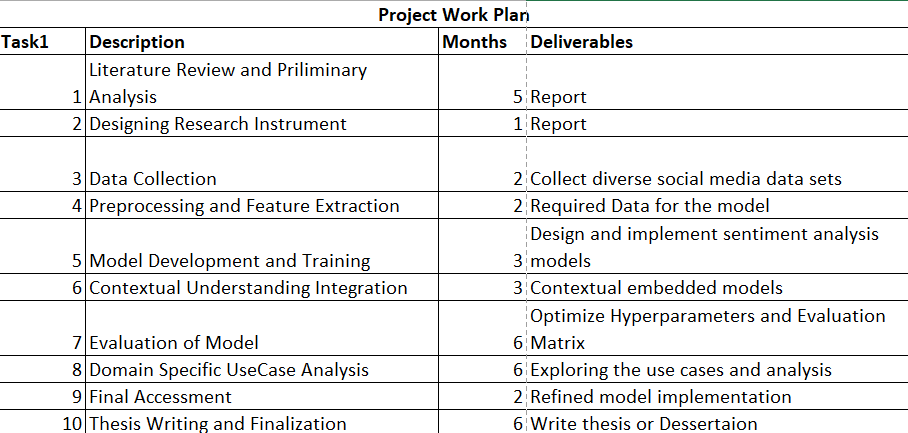
\includegraphics[width=\linewidth]{./workPlan1.png}
    \caption{Work Plan for Email Spam Detection Project}
    \label{fig:workPlan}
\end{figure}

\vspace{15pt}
\begin{figure}[H]
    \centering
    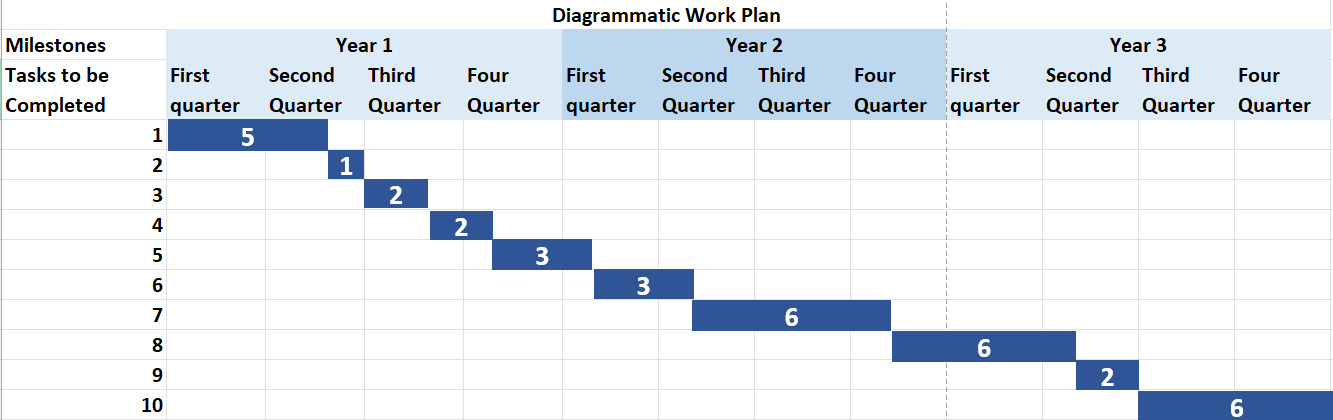
\includegraphics[width=\linewidth]{./workPlan2.png}
    \caption{Work Plan for Email Spam Detection Project}
    \label{fig:workPlan}
\end{figure}

\end{document}

